\chapter{Corner Regions and Additional Procedures}\label{ch:Modelling}
In this chapter we will introduce corner regions as an essential concept of this work and talk
about the additions we made to the corner detection algorithm in order to select the most valuable
corners for our inpainting mask.\\
The initial corner detection algorithm as well as the code for the inpainting algorithm was given
to me by courtesy of Joachim Weickert.

\section{Disk-shaped Corner Regions}
As mentioned in the beginning, the main concern for the approach of Zimmer~\cite{zimmer07}, alongside 
MCM not being suitable for inpainting, was that the corner localisation was not accurate enough that 
We can just keep a 4 or 8-neighbourhood of pixels.
The implication is that the regions he inserted into the mask were were too small to
cover the potential uncertainty in the corner localisation process stemming from the Gaussian
smoothing in the computation of the structure tensor (see Section~\ref{sec:Structure}). Specifically
because in order to limit the amount of corners detected, Zimmer chose to vary the integration scale
parameter increasing the uncertainty in the localisation, this poses a problem.
Hence, we want to explore increasing the neighbourhood of pixels that is kept around each
corner. A disk-shaped neighbourhood or \textit{(disk-shaped) corner region} with radius $r$ and origin point $(x, y)$ is defined as 
\begin{equation}
    B_r(x, y) = \lbrace (x',y') \in \Omega\ \vert\ {(x'-x)}^2 + {(y'-y)}^2 \leq r^2\rbrace
\end{equation}
The optimal choice for the radius of the corner disks is discussed in
Section~\ref{sec:ParameterSelection}.
Increasing the radius of the corner regions obviously leads to denser masks if one does not adjust
the limit of corner regions that are put in the mask. Since doing this manually for every picture
would not be practical at all in the context of a codec, we have to come up with a way to make sure
the resulting masks are always similar in pixel density.\newpage\noindent
One way to achieve this would be to introduce a percentile parameter instead of using the constant
threshold from the corner detection method described in~\ref{sub:Corner}.

\section{Percentile Thresholding}\label{sec:Percentile}
In the classic version of Harris corner detection, an artificial threshold parameter $T$
is introduced to weed out `bad' corners, i.e.\ corners where the \linebreak 
Harris measure~\eqref{def:Harris} is low. 
This parameter, however, is fairly sensible to the input image.\\
As a workaround to make this parameter a bit more robust, a percentile
parameter is introduced that is in turn used to compute a more robust threshold.\\
In statistics, the \textit{n-th percentile} of a set is the value that is larger than $n$ percent
of all values in this set.
We computed the percentile using the \textit{nearest-rank method} since this was the easiest
approach and worked good enough already. In this method, the n-th percentile is just simply
computed as the value at position 
\begin{equation} 
    \left\lceil \frac{n}{100}\cdot N_{x}N_{y}\right\rceil 
\end{equation} 
of the ordered set of values~\cite{percentile}.\\
Since in an image, there are more non-corners than actual corners, we have to deal with many zero
or close-to-zero cornerness values. This is a problem because the percentile computation would be skewed
heavily if e.g.\ more than 80 percent of all values are zero already. To solve this, we first filtered
out all values below a threshold close to zero and then accumulated the remaining values into an
array of appropriate size. This array is then sorted using an already implemented Quicksort
algorithm from the C standard library.\\
Subsequently, the new threshold is given as the value at the index calculated above.
While this approach works a bit better than the original version using the fixed threshold, it is
still not perfect. For example, if one uses a percentile of $0.5$, meaning that 
$50\%$ of all corners are thrown out, one could still get wildly different results 
for two different input images as we can see in~\ref{fig:PercExample}.
\begin{figure}[h!]
    \centering
    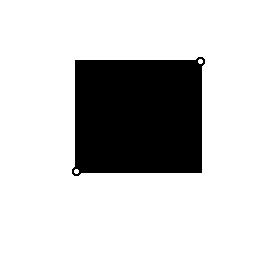
\includegraphics[width=0.4\linewidth]{example_rect_50.png}
    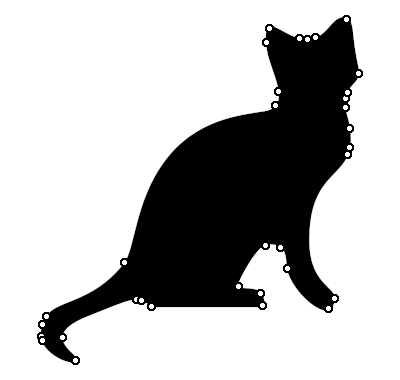
\includegraphics[width=0.4\linewidth]{example_cat_50.png}
    \caption{Corner detection with the same parameters. Parameters are $\sigma=1,\rho=2,q=0.3$, no
    CNMS, no TPPT}\label{fig:PercExample}
\end{figure}\\
To tackle this issue, we propose a new method that we call \textit{Total Pixel Percentage
Thresholding}. The idea behind this method is that one makes the amount of corners that are kept
in the masks dependent on the mask radius, i.e.\ the radius of a corner region in the inpainting
mask.\newpage\noindent
In other words, one specifies the desired mask pixel density and depending on the mask
radius, the maximum number of corners that can be inserted into the mask is
calculated.
The problem of calculating the number of pixels inside a disc of radius $r$ is also known as
\textit{Gauss' circle problem}~\cite{gaussCircle}. The exact solution to this problem is given
by~\cite{hilbert96}
\begin{equation}
    N(r) = 1 + 4\sum_{i=0}^{\infty}\left(\left\lfloor\frac{r^2}{4i+1}\right\rfloor - \left\lfloor
    \frac{r^2}{4i+3}\right\rfloor\right)
\end{equation}
but since this is an infinite sum, the exact solution can not be computed this way. This is why we
chose the naive way by just iterating through a loop and count the pixels inside the disk.
We could have also chosen to use an upper bound and estimate the number of pixels that 
way, but this would not have been as accurate.\\
After computing the area occupied by a single corner region we can simply calculate an upper bound on the number of
regions that can be inserted into the mask without exceeding the pixel density threshold by the equation
\begin{equation}
    N_{corners} = \left\lceil \frac{q \cdot N_{x}N_{y}}{N_{disc}} \right\rceil,\qquad0\leq q\leq 1 
\end{equation}
where $q$ is the percentile parameter, $N_x, N_y$ the number of pixels in the respective direction
and $N_{disc}$ the amount of pixels per corner region. 
Using this method, the pixel density of inpainting masks can be consistently recreated, as we will
see in the next chapter where we will present some examples of this method in
action.\newpage\noindent
Note that we did not consider the potential overlap of corner regions inside the
computation of $N_{disc}$, which is why this is only an upper bound, since there would have been no 
easy way to determine the amount of overlapping pixels a priori.\\
Instead, we introduced another method tackling the issue of potentially overlapping corner regions
called \textit{Circular Non-Maximum Suppression}. We will see how this method
works in the next Section~\ref{sec:Suppression}.
Another noteworthy point is that the amount of pixels in the mask using this approach is limited by
the number of corners detected since we do not even consider pixels that have a sufficiently small
cornerness value as mask candidates.
\section{Circular Non Maximum Suppression}\label{sec:Suppression}
\begin{figure}[t]
    \begin{lstlisting}[language=Python]
# Circular non-maximum suppression at x with radius r.
# Parameters:
#    -harris: Harris measure map
#    -x: current location as tuple
#    -r: radius of corner regions
#    -out: map of accepted corners after suppression
def circular_suppression(harris, x, r, out):
    for y in circle(x, r):
        if harris[y] > harris[x]:
            # The current location is not a maximum
            out[x] = 0
            return
    # Current location is a maximum, keep the region around it
    out[x] = harris[x]
    \end{lstlisting}
    \caption{Pseudo-Code for circular non-maximum suppression}
\end{figure}
\noindent As mentioned previously, overlapping corner regions tend to worsen the estimation of the mask pixel
density. 
Furthermore, as Zimmer~\cite{zimmer07} already stated, the sparsity of corners in images poses a
problem for the reconstruction quality. Circular non-maximum suppression is supposed to tackle both of these 
issues by increasing the radius of the local maximum search during the corner detection. 
In the original corner detection method, corners are determined by the local maxima inside an 
8-neighbourhood of the cornerness measure. The idea is to adapt the radius of the neighbourhood for the
local maximum search to the mask radius.\newpage\noindent
As experiments showed (see Section~\ref{sec:Results}), this minimises the overlap in
corner regions in the final mask and enables a fairly accurate estimation of the mask pixel
density, allowing us to consistently produce masks with similar density.
The other issue that this method tries to solve is the uneven distribution of corners across
the whole image. When limiting the amount of corners that are selected as candidates for the mask, one should not only care about
the `cornerness' of a corner, but also about its position. 
In other words, if a lot of good corners
are in close proximity to each other, it would be better to choose the ones that encase the 
highest number of `good' corners around them. 
That way, we get multiple corners `for the price of one' and can still introduce some 
of the `worse' corners to the mask.
By minimising the overlap between corner regions through this circular non-maximum suppression, we
can actually eliminate corners that are already covered by another disk from `a better' corner and
thus free up some slots for corners that may otherwise not have been selected for being sub-par.\\
One should note that this is not a perfect solution as certain constellations of corners create
an edge case in which a corner that is assumed to cover another corner is removed for being in the
disk of a better corner. This leads to the case where the corner that was formerly assumed to be
covered is suddenly not covered anymore and disappears from the mask without replacement, so future
work might be invested into finding a better solution for this approach.

